\documentclass{lib/myskripsi}

\usepackage{blindtext}

\renewcommand{\baselinestretch}{1.42}
\renewcommand{\UrlFont}{\small\rm}


%=============================================================================
% Package Daftar Pustaka, bentuk citasi
% Config
% - style, citestyle = {authoryear, numeric, apa, mla}
% - sorting {year,name,title} = ynt
%-----------------------------------------------------------------------------
\usepackage[
    backend=biber,
    style=authoryear,
    citestyle=authoryear,
    sorting=nty,
    giveninits=false,
    maxbibnames=3
    ]{biblatex}
\addbibresource{bibtex/daftar-pustaka.bib}
% new citation style
\let\oldcitate\cite
\newcommand*\thecite[1]{(\citeauthor{#1}, \citeyear{#1})}
%-----------------------------------------------------------------------------
% End Biblatex Config
%=============================================================================


%=============================================================================
% Definisi Data Peneliti, Judul, Pembimbing dan Penguji
%-----------------------------------------------------------------------------
\titleind{IMPLEMENTASI FILTER SPASIAL LINEAR PADA VIDEO \textit{STREAM} MENGGUNAKAN \textit{FPGA HARDWARE ACCELERATOR}}

\fullname{SULAEMAN}
\idnum{H131 16 002}

\examdate{\hspace{0.4cm} Mei 2020}
\yearsubmit{2020}

\degree{Sarjana Sains}
\program{Ilmu Komputer}
\dept{Matematika}
\faculty{Fakultas Matematika dan Ilmu Pengetahuan Alam}

\firstsupervisor{Dr. Eng. Armin Lawi, S.Si., M.Eng.}
\firstsupervisorNIP{94199834743819}
\secondsupervisor{Dr. Diaraya, M.Ak.}
\secondsupervisorNIP{32399834738431}
\firstexaminer{ Dr. Hendra, S.Si., M.Kom.}
\secondexaminer{ Nur Hilal A Syahrir, S.Si., M.Si.}
%-----------------------------------------------------------------------------
% End Definisi Data Peneliti, Judul, Pembimbing dan Penguji
%=============================================================================

\begin{document}
    % Halaman Sampul
    \coverproposal
    \pagenumbering{roman}

    % Halaman Judul
    \titlepage
    % Halaman Pernyataan Keotentikan
    \authenticationpage
    % Halaman Persetujuan Pembimbing
    \supervisorapprovalpage
    % Halaman Pengesahan
    \approvalpage

    % Kata Pengantar
    \addcontentsline{toc}{chapter}{KATA PENGANTAR}
    \chapter*{KATA PENGANTAR}

\blindtext
    \newpage

    % Pernyataan Persetujuan Publikasi Karya Ilmiah untuk Kepentingan Akademik
    \addcontentsline{toc}{chapter}{PERSETUJUAN PUBLIKASI ILMIAH}
    \chapter*{PERNYATAAN PERSETUJUAN PUBLIKASI TUGAS AKHIR UNTUK KEPENTINGAN AKADEMIK}

\blindtext
    \newpage

    % Abstrak
    \addcontentsline{toc}{chapter}{ABSTRAK}
    \chapter*{ABSTRAK}

\blindtext
    \newpage

    % Abstract
    % \addcontentsline{toc}{chapter}{ABSTRAK}
    \input{include/halaman-abstract.tex}
    \newpage



    %=============================================================================
    % Daftar isi, daftar gambar, daftar tabel
    %-----------------------------------------------------------------------------
    \tableofcontents
    \addcontentsline{toc}{chapter}{DAFTAR ISI}
    \newpage

    \listoftables
    \addcontentsline{toc}{chapter}{DAFTAR TABEL}
    \newpage

    \listoffigures
    \addcontentsline{toc}{chapter}{DAFTAR GAMBAR}
    \newpage
    %-----------------------------------------------------------------------------
    % End Daftar isi, daftar gambar, daftar tabel
    %=============================================================================


    \pagebreak
    \pagenumbering{arabic}


    %=============================================================================
    % Daftar masukan untuk Bab
    %-----------------------------------------------------------------------------
    \chapter{PENDAHULUAN}

\section{Latar Belakang}

\blindtext 
\thecite{book:darma}
    
\chapter{TINJAUAN PUSTAKA}


\section{Landasan Teori}

\subsection{Citra Digital}
Citra digital dapat didefinisikan sebagai fungsi f(x,y) berukuran M baris dan N kolom, dengan x dan y adalah kordinat spasial, dan amplitudo f di titik kordinat (x,y) dinamakan intensitas atau tingkat keabuan dari citra pada citra tersebut \thecite{book:darma}. Pada umumnya warna dasar dalam citra RGB menggunakan penyimpanan 8 bit untuk menyimpan data warna, yang berarti setiap warna mempunyai gradasi sebanyak 255 warna . Dewasa ini, citra digital dapat menggunakan 16 bit untuk menyimpan data warna dasarnya, hal ini menyebabkan semakin banyak gradasi warnanya sehingga citra yang dihasilkan memiliki tingkat warna yang jauh lebih banyak. Namun tentu saja hal ini mengakibatkan ukuran file citra digital yang dihasilkan juga menjadi semakin besar walaupun dengan resolusi yang sama. Berdasarkan jenis warnanya citra digital dibagi menjadi 3 jenis:

\begin{enumerate} [label=\textbf{\alph*.}]
    \item \textbf{Citra Biner (Monokrom)} \\ 
    Banyaknya dua warna, yaitu hitam dan putih. Warna hitam direpresentasikan dengan 1 dan warna putih direpresentasikan dengan 0. Dibutuhkan 1 bit di memori untuk menyimpan warna ini. Contoh citra biner dapat dilihat pada gambar ~\ref{fig:jenis-citra}(a).
    \item \textbf{Citra Grayscale (Skala keabuan)} \\ 
    Banyaknya warna tergantung pada jumlah bit yang disediakan di memori untuk menampung kebutuhan warna ini. Citra 2 bit mewakili 4 warna, citra 3 bit mewakili 8 warna, dan seterusnya. Semakin besar jumlah bit warna yang disediakan di memori, semakin halus gradasi warna yang terbentuk. Pada umumnya citra digital grayscale menggunakan 8 bit memori dengan derajat keabuan dari 0 sampai 255. Contoh citra grayscale dapat dilihat pada gambar ~\ref{fig:jenis-citra}(b).
    \item \textbf{Citra Warna} \\ 
    Setiap piksel pada citra warna mewakili warna yang merupakan kombinasi dari tiga warna dasar (RG8 = Red Green Blue). Setiap warna dasar menggunakan penyimpanan 8 bit, yang berarti setiap warna mempunyai gradasi sebanyak 255 warna. Berarti setiap piksel mempunyai kombinasi warna sebanyak 255 x 255 x 255 =16 juta warna lebih. Dibutuhkan 3x8 = 24 bit di memori untuk menyimpan sebuah data warna ini. Contoh citra warna dapat dilihat pada gambar ~\ref{fig:jenis-citra}(c).
\end{enumerate}

\begin{afigure}
    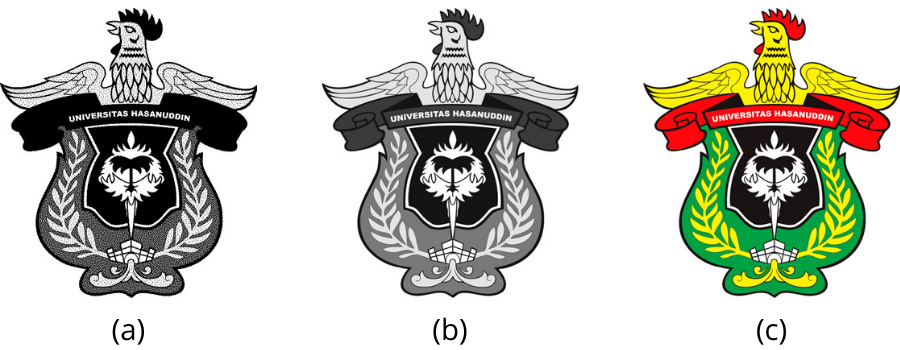
\includegraphics[width=1\textwidth, center]{images/jenis-jenis-citra.png}
    \caption{(a) Contoh citra biner, (b) contoh citra grayscale, (c) contoh citra warna.}
    \label{fig:jenis-citra}
\end{afigure}


\subsection{Pengolahan Citra Digital}
Pengolahan citra digital merupakan proses mengolah piksel-piksel di dalam citra digital untuk tujuan tertentu. Berdasarkan tingkat pemrosesannya pengolahan citra digital dikelompokkan menjadi tiga kategori, yaitu: \textit{low-level}, \textit{mid-level} dan pemrosesan \textit{high-level}. Pemrosesan \textit{low-level} dilakukan dengan operasi primitif seperti \textit{image preprocessing} untuk mengurangi derau (\textit{noise}), memperbaiki kontras citra dan mempertajam citra (\textit{sharpening}). Karakteristik dari pemrosesan \textit{low-level} yaitu keluaran atau hasil dari pemrosesannya berupa citra digital. Pemrosesan \textit{mid-level} melibatkan tugas-tugas seperti segmentasi (mempartisi gambar menjadi beberapa bagian atau objek), deskripsi objek untuk dilakukan pemrosesan lanjutan, dan klasifikasi objek dalam citra digital. Karakteristik dari pemrosesan \textit{mid-level} yaitu keluaran atau hasilnya berupa atribut atau fitur seperti, kontur, tepi, atau objek yang terdapat dalam citra tersebut. Pemrosesan \textit{high-level} merupakan proses tingkat lanjut dari dua proses sebelumnya, dilakukan untuk mendapat informasi lebih yang terkandung dalam citra \thecite{book:gonzalez}.

\subsection{Filter Spasial}
Konsep filter bersumber dari penerapan transformasi Fourier untuk pemrosesan sinyal pada domain frekuensi. Istilah filter spasial ini digunakan untuk membedakan proses ini dengan filter pada domain frequensi. Proses filter spasial ini dilakukan dengan cara menggeser filter kernel dari titik ke titik dalam citra digital. Istilah mask, kernel, template, dan window merupakan isitilah yang sama dan sering digunakan dalam pengolahan citra digital \thecite{book:gonzalez}. Dalam penelitian ini penulis menggunakan istilah kernel untuk istilah tersebut.
% Rumusnya
% rumusnya bisa dilihat pada \ref{eq:conv}
% Perbedaan Filter Linear dan Non Linear
Konsep filter spasial linear mirip seperti konsep konvolusi pada domain frekuensi, dengan alasan tersebut filter spasial biasa disebut juga konvolusi sebuah kernel dengan citra digital \thecite{book:gonzalez}.

Konvolusi dua buah fungsi f(x) dan g(x) didefenisikan sebagai berikut:

\begin{equation}
    \label{eq:conv}
    \begin{split}
        h(x) &= f(x)*g(x) \\
        &= \int_{-\infty}^{\infty}f(a)g(x-a) da
    \end{split}
\end{equation}
% The subimage is called a filter, mask, kernel, template, or window, with the first three terms being the most prevalent terminology. 

% As discussed in Chapter 4, the process of linear iltering given in Eq. (3.5-1) is similar to a frequency domain concept called convolution. For this reason, linear spatial filtering often is referred to as  convolving a mask with an image.” Similarly, filter masks are sometimes called  onvolution masks. The term con- volution kernel also is in common use. 

\subsection{Video Streaming}
Video stream dapat dipandang sebagai serangkaian citra digital berturut-turut \thecite{thesis:jin}. Berbeda dengan format video lainya, video stream ini tidak disimpan pada media penyimpanan sebagai file video melainkan langsung disalurkan setiap framenya dari sumber (source) ke penerima, dalam hal ini FPGA.  Dengan menganggap Video stream adalah kumpulan citra digital (frame) maka dapat dilakukan metode pengolahan seperti pada citra digital, termasuk filter spasial. 

\subsection{FPGA}
Field Programmable Gate Arrays atau FPGA adalah perangkat semikonduktor yang berbasis \textit{matriks configurable logic block} (CLBs) yang terhubung melalui interkoneksi yang dapat diprogram.

FPGA dapat diprogram ulang ke aplikasi atau fungsi yang diinginkan setelah \textit{manufacturing}. Fitur ini yang membedakan FPGA dengan \textit{Application Specific Integrated Circuits} (ASICs), yang dibuat khusus untuk tugas tertentu saja \thecite{XILINX}.

Sebuah \textit{microprocessor} menerima instruksi berupa kode 1 atau 0, kode-kode ini selanjutnya diinterpretasikan oleh komputer untuk menjalankan perintah yang diberikan. \textit{Microprocessor} ini membutuhkan intruksi berupa kode secara terus menerus untuk menjalankan fungsinya. Sedangkan pada FPGA hanya dibutuhkan sekali konfigurasi \textit{chip} setiap kali dinyalakan. Membuat atau mengunduh \textit{bitstream} yang menentukan fungsi logika dilakukan oleh \textit{logic elements} (LEs), sebuah sirkuit dapat dibuat dengan mengabungkan beberapa LEs menjadi satu kesatuan. Setelah \textit{bitstream} dipasang, FPGA tidak perlu lagi membaca instruksi berupa 1 dan 0, berbeda dengan \textit{microprocessor} yang selalu membutuhkan instruksi \thecite{pdf:cheung}.

\begin{afigure}
    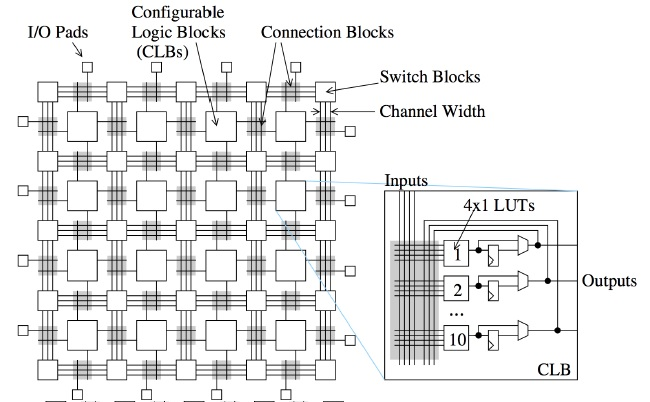
\includegraphics[width=12cm, center]{images/fpga-structure.jpeg}
    \caption{Struktur FPGA.}
    \label{fig:fpga-structure}
\end{afigure}



\subsection{Tepi Citra}
Suatu titik (x, y) pada citra digital dikatakan sebagai tepi apabila perubahan nilai intensitas derajat keabuan yang mendadak (besar) dalam jarang yang berdekatan. Tepi biasanya terdapat pada batas andara dua daereah yang berbeda pada suatu citra. Tepi pada citra dapat merepresentasikan objek-objek yang terkandung dalam citra tersebut, bentuk dan ukurannya atau terkadang juga informasi tentang teksturnya.

Tepi citra dapat dilihat melalui perubahan intensitas pixel pada suatu area. Berdasarkan perbedaan perubahan intensitas tersebut, tepi dapat dibagi menjadi 4 jenis yaitu tepi steep, ramp, line dan step-line \thecite{book:darma}.

\begin{enumerate} [label=\textbf{\alph*.}]
    \item \textbf{Steep}, tepi jenis \textit{step} merupakan tepi citra yang berbentuk dari perubahan intensitas nilai pixel secara signifikan dari tinggi ke rendah ataupun sebaliknya.
    \item \textbf{Ramp}, tepi jenis ini terbentuk dari perubahan intensitas nilai pixel secara perlahan. Perubahan secara perlahan dapat dilihat pada bentuk kurva yang semakin tinggi dengan perubahan kontinu.
    \item \textbf{Line}, tepi jenis ini ditandai dengan perubahan intensitas nilai pixel secara drastis dari rendah-tinggi-rendah atau sebaliknya.
    \item \textbf{Step-Line}, tepi \textit{step-line} merupakan gabungan dari tepi jenis step dan line. Tepi jenis ini ditandai dengan peningkatan intensitas yang tajam dalam interval tertentu dan kemudian ditandai dengan penurunan yang tidak signifikan, sehingga perubahan intensitas nilai pixel selanjutnya berlangsung stabil.
\end{enumerate}

% Tambahkan gambar 

% halaman 201
% https://books.google.co.id/books?hl=en&lr=&id=NectMutqXJAC&oi=fnd&pg=PR4&dq=buku+pengolahan+citra+digital&ots=C2oB2TDTo4&sig=UnkxuezGlrECiOZBepXOMa__gEY&redir_esc=y#v=onepage&q=buku%20pengolahan%20citra%20digital&f=false


\subsection{Deteksi Tepi}
Deteksi tepi merupakan salah satu metode dalam pemrosesan cira digital untuk deteksi fitur dan ekstraksi dengan mengidentifikasi titik-titik (pixel) dalam citra yang mengalami perubahan tingkat keabuan secara derastis dan mengalami diskontinu. Salah satu tujuan deteksi tepi yaitu untuk mengurangi jumlah data secara signifikan dalam suatu gambar dan mempertahankan sifat strukturalnya untuk pemrosesan citra lebih lanjut. \thecite{desi_herawati}.

Berbagai macam metode deteksi dapat digunakan untuk mendeteksi tepi pada citra. Setiap teknik memiliki keunggulan dan karakteristiknya masing-masing. Suatu teknik deteksi tepi mungkin dapat bekerja sangat baik dalam suatu aplikasi tertentu namun sebaliknya belum tentu dapat berjalan secara maksimal pada aplikasi lainnya.

Terdapat berbagai operator deteksi tepi yang telah dikembangkan berdasarkan turunan pertama (first order derrivate), di antaranya operator Robert, operator Sobel, operator Prewitt, operator Krisch, dan operator Canny. Konsep dasar dari deteksi tepi dengan turunan pertama adalah dengan memanfaatkan perbedaan nilai suatu pixel dengan pixel tetangganya. 
% operator turunan kedua, dan seterusnya


\section{Penelitian Terkait}
\subsection{Spatial Filtering Based Boundary Extraction in Underwater Images for Pipeline Detection: FPGA Implementation}
\blindtext \thecite{soa:alex-raj}

\subsection{FPGA Implementation of Spatial Filtering techniques for 2D Images}
\blindtext \thecite{soa:sushant}

\subsection{Features of Image Spatial Filters Implementation on FPGA}
\blindtext \thecite{soa:dmitry}

\subsection{An FPGA-Oriented Algorithm for Real-Time Filtering of Poisson Noise in Video Streams, with Application to X-Ray Fluoroscopy}
\blindtext \thecite{soa:castellano}

\subsection{A real-time video denoising algorithm with FPGA implementation for Poisson-Gaussian noise}
\blindtext \thecite{soa:xin}

    
\chapter{METODE PENENILITIAN}


\section{Tahapan Penelitian}
Tahapan dalam penelitian ini dapat dilihat pada gambar \ref{fig:penelitian-flowchart}.
\begin{afigure}
    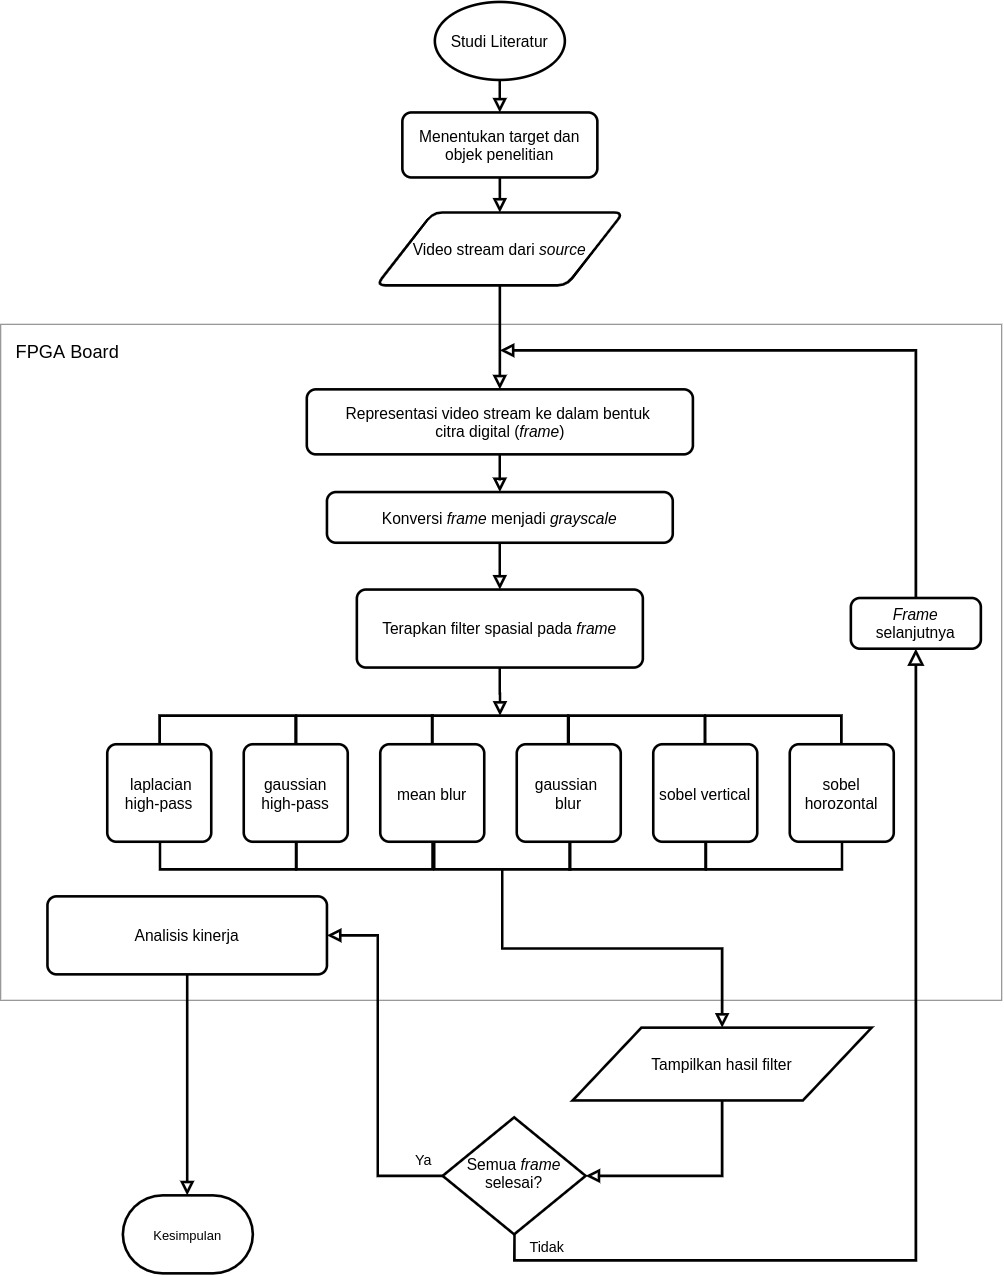
\includegraphics[width=13cm, center]{images/penelitian-flowchart.jpg}
    \caption{Flowchart tahapan penelitian.}
    \label{fig:penelitian-flowchart}
\end{afigure}
% tambahkan penjelasan lagi


\section{Waktu dan Lokasi Penelitian}
Penelitian ini dilaksanakan dari bulan Juni 2020 sampai dengan bulan Agustus 2020. Lokasi penelitian dilakukan di Laboratorium Rekayasa Perangkat Lunak Fakultas Matematika dan Ilmu Pengetahuan Alam, Universitas Hasanuddin Makassar.

\section{Rancangan Sistem}
Pada penelitian ini akan dibangun suatu sistem untuk mengimplementasikan filter spasial linear pada FPGA, dapat dilihat pada gambar \ref{fig:rancangan-sistem}.
\begin{afigure}
    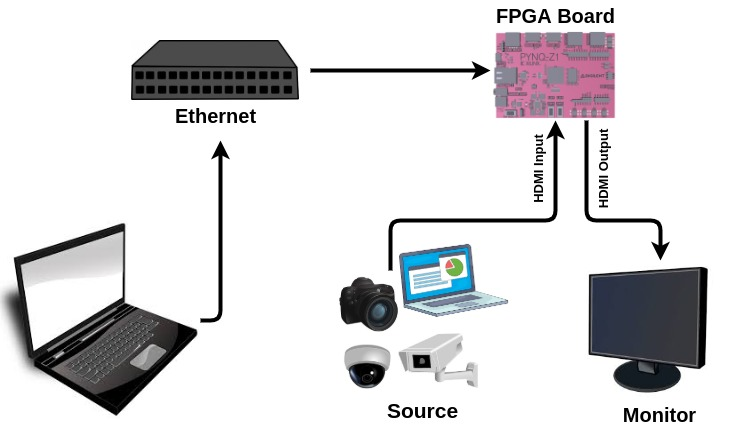
\includegraphics[width=0.85\textwidth, center]{images/rancangan-sistem.jpg}
    \caption{Rancangan sistem.}
    \label{fig:rancangan-sistem}
\end{afigure}

Video stream dari \textit{source} akan disalurkan melalui port HDMI Input pada FPGA Board, kemudian video stream tersebut akan diolah dengan menerapkan filter spasial linear pada setiap framenya. Setiap frame yang telah dilakukan filter spasial akan dialirkan ke monitor untuk kemudian ditampilkan. Selanjutnya dilakukan analisis kinerja pada FPGA. FPGA board yang digunakan dalam penelitian ini dapat diakses dengan \textit{ssh} pada port 22 atau dengan Jupyter Notebook melalui browser.

\section{Instrumen Penelitian}
Instrumen penelitian ini yaitu:
\begin{enumerate}[topsep=0pt,itemsep=0pt,partopsep=0pt, parsep=0pt]
    \item Kebutuhan perangkat lunak:
    \begin{enumerate}[topsep=0pt,itemsep=0pt,partopsep=0pt, parsep=0pt, label={\alph*.}]
        \item Ubuntu 16, sebagai OS pada FPGA Board
        \item Python 3.6 (dengan modul OpenCV dan Numpy)
        \item Jupyter Notebook, sebagai interface untuk mengakses FPGA Board 
        % \item Chrome Browser 
    \end{enumerate}
    \item Kebutuhan perangkat keras:
    \begin{enumerate}[topsep=0pt,itemsep=0pt,partopsep=0pt, parsep=0pt, label={\alph*.}]
        \item FPGA Board Xilinx PYNQ-Z2
        \item Micro SD Card 8Gb (sebagai media penyimpanan OS pada FPGA Board)
        \item Monitor Eksternal (untuk menampilkan hasil filter dari FPGA)
        \item Laptop Lenovo Ideapad 320 (sebagai source video stream)
        \item 2 buah kabel HDMI (untuk HDMI input dan HDMI output pada FPGA) 
    \end{enumerate}
\end{enumerate}

    
\chapter{HASIL DAN PEMBAHASAN}

% \section{}
% \section{Cara Implementasi}
% \section{Kinerja FPGA}


% cara implementasi
% perbandingan hasil

% \section{}
% \subsection{Citra Digital}

% video stream sebagai citra
% penerapan filter spasial
% - - - -
% Analisis Kinerja





    
\chapter{KESIMPULAN DAN SARAN}


\section{Kesimpulan}
% \subsection{Citra Digital}
\blindtext

\section{Saran}
\blindtext
    %-----------------------------------------------------------------------------
    % End Daftar masukan untuk Bab
    %=============================================================================


    %=============================================================================
    % Daftar Pustaka
    % %-----------------------------------------------------------------------------
    \addcontentsline{toc}{chapter}{DAFTAR PUSTAKA}
    \printbibliography[title={DAFTAR PUSTAKA}]
    %-----------------------------------------------------------------------------
    % End Daftar Pustaka
    %=============================================================================

    % Lampiran
    \addcontentsline{toc}{chapter}{LAMPIRAN}
    \chapter*{LAMPIRAN}

\blindtext

% \subsection*{Percobaan 1}

\begin{small}
    % \caption{Perbandingan FPS}
    \label{table:arm-aveblur1}
    \csvreader[
        % column count = 11,
        head to column names,
        longtable=cccccccc,
        separator=semicolon,
        before table=\rowcolors{2}{gray!15}{gray!30},
        table head= \rowcolor{gray!50!black} 
            \color{white} PID & 
            \color{white} VIRT & 
            \color{white} RES &
            \color{white} SHR & 
            \color{white} Status &  
            \color{white} CPU(\%) &
            \color{white} MEM(\%) & 
            \color{white} Time(s) 
            \\]
        {tables/performance-test/arm-aveblur5.csv}
        {
            PID=\PID, 
            VIRT=\VIRT, 
            RES=\RES,
            SHR=\SHR, 
            S=\S,
            CPU=\CPU,
            MEM=\MEM, 
            TIME=\TIME}
        {
            \PID & 
            \VIRT & 
            \RES &
            \SHR & 
            \S &
            \CPU &
            \MEM & 
            \TIME}
\end{small}

\end{document}
